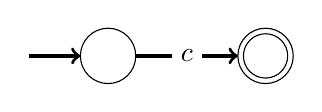
\begin{tikzpicture}[
  vertex/.style = {
    shape = circle,
    draw = black,
    minimum size = 20pt,
    inner sep = 0pt,
    outer sep = 0pt,
  }
]
  \node[vertex] (v1) at (2, 0) {};
  \node[vertex] (v2) at (4, 0) {};

  \draw (4, 0) circle (8pt);  

  \begin{scope}[every path/.style = { very thick }]
    \draw[->] (1, 0) -- (v1);
    \draw[->] (v1) -- (v2) node[midway, sloped, fill = white] {\(c\)};
  \end{scope}
\end{tikzpicture}
